
\section{Problem}

Now that we have established our methodology for sensing the free space of the environment, we need some way of integrating our local free space maps into a map representation.  At each anchored position between locomotion steps, we create two free space maps for the front and back probe sweeps respectively.  Each local map is plotted in a local coordinate frame centered on the middle of the robot.  These local maps created while the robot is traveling through the environment need to be stitched together to make a global map.

We develop an approach to build a map using a \emph{pose graph} representation [cite].  We explain our specific implementation in the next section and demonstrate the results of our approach.

\section{Pose Graph Representation}

Our approach is derived from Pose/Feature Graphs [Olson2008] but differs in that we do not have feature nodes.  Since we only have pose nodes, we call it a Pose Graph.  This is similar to other graph-based approaches such as Constraint Networks, Graph-Based SLAM or Network-Based SLAM.

\begin{figure}
  \begin{center}
    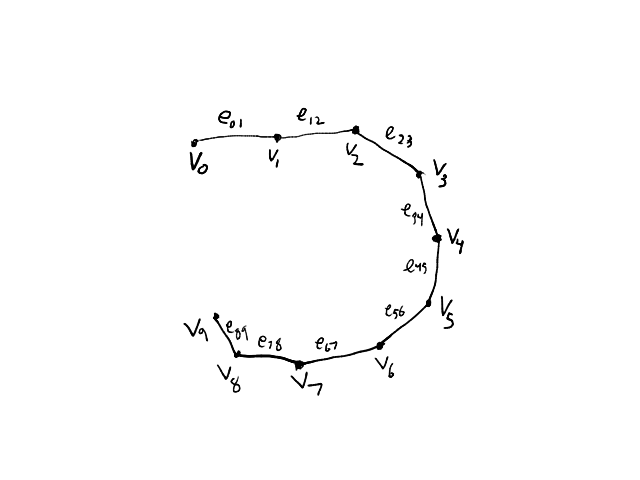
\includegraphics[scale=0.7]{5_pose_graph_basic.png}
  \end{center}
  \caption{Simple Pose Graph}
  \label{fig:simple_pose_graph}
\end{figure}

A pose graph is defined by a set of nodes $V$ and a set of edges $E$.  Each node $v_k \in V$ represents a position of the robot in the environment and its collected sensor data.  Each edge $e_{ij} \in E$ represents a geometric relation between the nodes $v_i$ and $v_j$.  A simple example is shown in Figure \ref{fig:simple_pose_graph}.

Each \textbf{node} $v_k \in V$ is associated with a corresponding pose $\hat{P_k}$ and local free space map $M_k$ created at that pose.  The pose is the location of the GPAC origin of the snake robot originally defined in Section \ref{sec:GPAC}.  The local map $M_k$ is the free space data originally defined in Chapter \ref{chap:sensing}.

Each \textbf{edge} $e_{ij} \in E$ is associated with a geometric transform $T_{ij}$ and a covariance matrix $C_{ij}$ between the nodes $v_i$ and $v_j$.  $T_{ij}$ represents the geometric transform between $\hat{P}_i$ and $\hat{P}_j$ and is derived from the motion estimation system as detailed in Section \ref{sec:geo_transform}.  Other derivations for the geometric transform are possible and are described in the next section.  The covariance $C_{ij}$ is represents the uncertainty of $T_{ij}$ between the two poses.  Together the $T_{ij}$ and $C_{ij}$ form a \emph{constraint}.
%The reason for the use of GPAC for our poses now becomes apparent as two consecutive poses will have similiar pose angles.

We add nodes and edges to the pose graph as the robot travels through the environment and collects sensor information.  We can later use a batch optimization algorithm to find the minimum error satisfaction of the constraints to produce a corrected map.  The correctness of the resultant map depends on the quality of the constraints.  That is, the correctness of the geometric transform $T_{ij}$ and an accurate representation of its uncertainty $C_{ij}$.

%As the pose graph is built, we can input the graph representation into a batch optimization algorithm that adjustes the poses of $V$ to produce a minimum error satisfaction of the constraints represented by the geometric transforms and uncertainties of $E$.  Since our current approach is in 2D, we use the freely available 2D network optimizer TORO [cite].  This will perform map correction so long as the constraints in the pose graph are chosen wisely.

At the end of each AdaptiveStep locomotion step, we create two new nodes for the robot snake's anchored position.  The two nodes represent the snake's forward sweeping behavior and backward sweeping behavior respectively.  Each node contains the local map created from the execution of a PokeWalls behavior shown in Figure \ref{ref_sweep_sep}.  If $k=n_v$ is the total number of nodes in the pose graph, the newly created nodes are $v^f_{k}$ and $v^b_{k+1}$ for the forward and backward sweeps respectively.  Our graph starts to look like in Figure \ref{fig:paired_pose_graph}.

\begin{figure}
  \begin{center}
    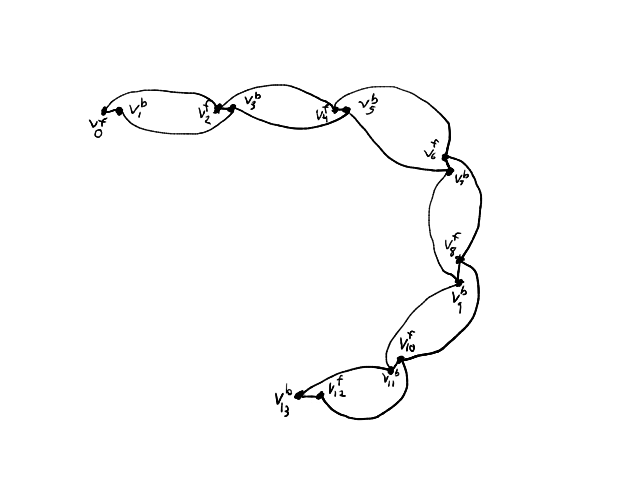
\includegraphics[scale=0.7]{5_pose_graph_paired.png}
  \end{center}
  \caption{Pose Graph from Paired Poses}
	\label{fig:paired_pose_graph}
\end{figure}

%To add \emph{nodes} to the pose graph, we create two after AdaptiveStep locomotion step is performed while the snake robot is anchored to perform its probe sweeping behavior.   One node is created for the forward sweep and the other is for the backward sweep.  Each node has two local maps that reflect the sensor results of the PokeWalls behavior as in Figure \ref{ref_sweep_sep}.  After the sensing phase is complete, the AdaptiveStep is performed again and the snake robot anchors once again.  Two more nodes are created and the process is continued ad infinitum for each stop after a locomotion step.

%The base condition at the start of mapping is that two nodes are created $v^f_0$ and $v^b_1$ which are forward and backward nodes respectively.  The next two nodes created are $v^f_{i}$ and $v^b_{i+1}$ where $i=n_v=2$, and $n_v$ is the total number of nodes previously created.

Edges are created when we have some knowledge about the geometric relation between nodes.  Care must be taken when choosing constraints so that we do not over-constrain or under-constrain the graph.  If an erroneous geometric constraint is added with an associated low uncertainty, this will result in a erroneous local minima in the constraint error minimization problem.  Conversely, if there are no constraints with low uncertainty, very little correction will occur.

%We create \emph{edges} to represent geometric constraints.  Our geometric constraints come from our motion estimation system as well as our assumptions about how the robot moves.  We do not want too few constraints or not enough information is present to perform any type of correction.  If we have too many constraints, then our system becomes over-constrained and no amount of further observation will correct it.

To show how we start to build the graph, given two consecutive pairs of nodes, $v^f_0, v^b_1, v^f_2, v^b_3$, we add the following edges to the graph: $e_{01}, e_{02}, e_{13}, e_{23}$.  The two constraints $e_{01}$ and $e_{23}$ we call in-place constraints since they apply to matched pairs of nodes that are in the same position but are probe sweeping different sides of the snake.  The two constraints $e_{02}$ and $e_{13}$ are motion constraints and are directly pulled from the relationship between GPAC poses in our motion estimation system.

The series of nodes begin to look like in Figure \ref{fig:paired_pose_graph}.  After application of the TORO network optimizer, it can perform limited corrections.   Further corrections are not yet possible because we have not discussed how to constrain nodes of the graph that overlap each other in space but not in time.  We can see that backtracking will create drift between disparate points of the maps in Figure \ref{fig:backtrack_pose_graph}.  We show how to correct this in the next chapter.

\begin{figure}
  \begin{center}
    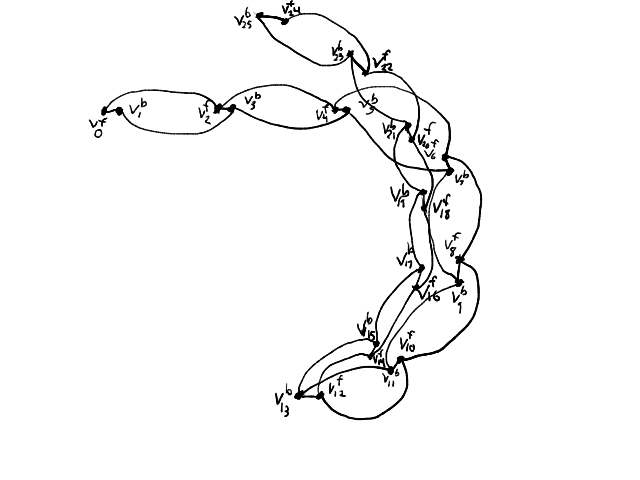
\includegraphics[scale=0.7]{5_pose_graph_backtrack.png}
  \end{center}
  \caption{Pose Graph with Uncorrected Backtracking}
	\label{fig:backtrack_pose_graph}
\end{figure}

Also, we show a plot of the local sweep maps into a global map with the optimized poses in Figure X.  Sometimes, it easier to see the map as a series of postures as in Figure \ref{fig:posture_plot}.


\begin{figure}
  \begin{center}
    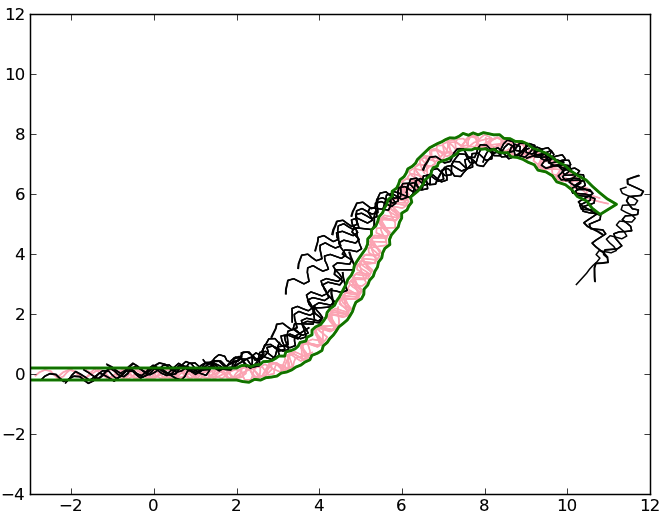
\includegraphics[scale=0.7]{plotMotionVariableWidth.png}
  \end{center}
  \caption{Postures at Nodes in the Graph}
	\label{fig:posture_plot}
\end{figure}



%Poses are represented with GPAC pose reference frames
%Reduces variance of angle, makes relevant, not noise


\section{Types of Constraints}

The next thing we establish is what kinds of constraints we apply to the pose graph and how they are derived.  Here, we discuss three different types of constraints.

The \emph{motion constraint} is derived from the motion estimation system we discussed in Chapter 3.  The \emph{in-place constraint} is a relationship between the forward and backward probe sweep nodes.  We also introduce the \emph{step constraint}, a simplified form of motion estimation that, under the right conditions, is a desirable replacement to the motion constraint.

\subsection{Motion Constraint}

The construction of the motion constraint is taken directly from the output of our motion estimation system.  That is, for each pose represented by the two nodes, we use the associated reference poses to compute the GPAC and its local frame origin.   The GPAC pose $\hat{P_k}$ for each node $v_k$ of the pose graph is computed by taking its reference pose $P_{19}$ at the time of its creation $t$, the joint posture $\bar{\phi}_t$, compute the segment posture $\bar{\rho_t}$, the GPAC function $\beta_t(u)$, and finally resulting in its global GPAC pose $\hat{P_k}$.  This process is detailed in Section \ref{sec:GPAC}.

The geometric offset $T_{02}$ between the two nodes $v^f_0$ and $v^f_2$, using Equations \ref{equ:g_to_c_cart} and \ref{equ:g_to_c_ori} and setting the respective GPAC poses to $P^g_a = \hat{P}_0$ and $P^g_b = \hat{P}_2$, gives us our transform in the form:
%\begin{equation}
%T_{02} = 
%\begin{bmatrix}
%x_{02} \\
%y_{02} \\
%\theta_{02}
%\end{bmatrix}
%\quad
%\left\{ 
%  \begin{array}{l l}
%    x_{02},y_{02} & \quad \text{from Equation \ref{equ:g_to_c_cart} }\\
%    \theta_{02} & \quad \text{from Equation \ref{equ:g_to_c_ori}}
%  \end{array} \right.
%\text{for $P^g_a = \hat{P}_0$ and $P^g_b = \hat{P}_2$}
%\end{equation}
%That is,
%\begin{equation}
%\begin{bmatrix}
%x_{02} \\
%y_{02} \\
%\end{bmatrix}
% = \hat{R_0}
%{\hat{G_0}}^{\mathbf{T}} \left(\hat{G_0}
%\begin{bmatrix}
%\hat{x_2} \\
%\hat{y_2}
%\end{bmatrix}
%-
%\begin{bmatrix}
%|(\hat{x_0},\hat{y_0})|\\
%0
%\end{bmatrix}
%\right)
%\end{equation}
%and
%\begin{equation}
%\theta_{02} = \theta_2 - \theta_0
%\end{equation}


\begin{equation}
T_{02} = 
\begin{bmatrix}
x_{02} \\
y_{02} \\
\theta_{02}
\end{bmatrix}
\quad
\left\{ 
  \begin{array}{l l}
\begin{bmatrix}
x_{02} \\
y_{02} \\
\end{bmatrix}
 = \hat{R_0}
{\hat{G_0}}^{\mathbf{T}} \left(\hat{G_0}
\begin{bmatrix}
\hat{x_2} \\
\hat{y_2}
\end{bmatrix}
-
\begin{bmatrix}
|(\hat{x_0},\hat{y_0})|\\
0
\end{bmatrix}
\right) \\
  \theta_{02} = \theta_2 - \theta_0
  \end{array} \right.
\end{equation}
where $\hat{R_0}$ is derived from Equation \ref{equ:coord1} and $\hat{G_0}$ is derived from Equation \ref{equ:coord4}.

%and
%\begin{equation}
%\end{equation}


The covariance of the constraint can be computed empirically by taking the mean and covariance of a large data set of estimated and ground truth constraints.  However, we assume that $x_{02}$, $y_{02}$, and $\theta_{02}$ are independent of each other, so their associated covariances are 0.  The covariance matrix we use for the motion constraint is the following:

\begin{equation}
C_{02} = 
\begin{bmatrix}
0.06 & 0 & 0 \\
0 & 5.0 & 0 \\
0 & 0 & 0.1 
\end{bmatrix}
\end{equation}

This matrix implies that the error along the x-axis direction (forward/backward) is less pronounced than the error along the y-axis (side-to-side) with a moderate amount of rotational error.  This particular matrix is a hand-made approximation of our observations of the error in the motion estimation.  We apply it to our motion constriants.

\subsection{In-Place Constraint}

The in-place constraint's role is to relate the forward and backward nodes of a single anchor position's probe sweeping.  Ideally, the transform between the two poses would be zero change.  However, our experience with the reference pose errors of Chapters 3 and 4 tell us that errors are always possible and likely.  Therefore, we provide a method of guessing a good in-place constraint, and present our hand-made covariance matrix to approximate the error. 

The naive approach would be to have a zero transform for our constraint of two nodes that are in the same place, such that:

\begin{equation}
T_{01} = 
\begin{bmatrix}
x_{01} \\
y_{01} \\
\theta_{01}
\end{bmatrix}
= 
\begin{bmatrix}
0 \\
0 \\
0
\end{bmatrix}
\end{equation}


However, the difference between the two poses must account for reference pose errors, slipping, and differences in the dynamic generation of their respective GPAC poses.  A clue to making this easier is to recognize that both postures of the forward and backward nodes should occupy the same space, and therefore should not be intersecting the walls of the environment that are likely there.  If we focus on making sure the postures of the snakes overlap each other as well as possible in space, we can compute the best fit transform between the two poses in place.

Again, we use B-splines to compute GPACs for both the forward and backward segment postures in the local coordinates.  We define these to be $\beta_0^f(u)$ and $\beta_1^b(u)$. However, instead of computing the GPAC pose by $\beta_0^f(0.5)$ and $\beta_1^b(0.5)$, we find the closest point on the GPACs to the local origin, $O_k$, discussed in Section \ref{sec:ref_stable}.  The closest point on the GPAC gives us a point and a direction represented by a pose $I_k$.  For nodes $v^f_0$ and $v^b_1$, this gives us $I_0$ and $I_1$ as shown in Figure \ref{fig:local_origin}.

We find $u_0$ and $u_1$ such that:
\begin{equation}
\beta_0^f(u_0) = I_0
\end{equation}
\begin{equation}
\beta_1^b(u_1) = I_1
\end{equation}

\begin{figure}
  \begin{center}
    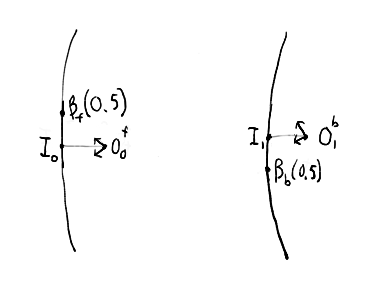
\includegraphics[scale=0.8]{5_local_origin.png}
  \end{center}
  \caption{Point $I_k$ on Curve $\beta_k$ from Local Origin $O_k$}
	\label{fig:local_origin}
\end{figure}

Our next step is to perform an iterative closest point (ICP) search of the two GPACs so that they overlap each other as closely as possible.  We use only a single variable search using the angle.  The two curves are placed on top of each other at the poses $I_0$ and $I_1$ so that the angles are aligned and the curves are tangent.  The ICP search finds the angular difference between $I_0$ and $I_1$ such that the ICP error between the two curves is minimized, shown in Figure \ref{fig:inplace_ICP}.

That is, we find the angle $\theta_v$ that minimizes the ICP cost while satisfying the following invariant condition:
\begin{equation}
I_1 = I_0 +
\begin{bmatrix}
0 \\
0 \\
\theta_v
\end{bmatrix}
\end{equation}

\begin{figure}
  \begin{center}
    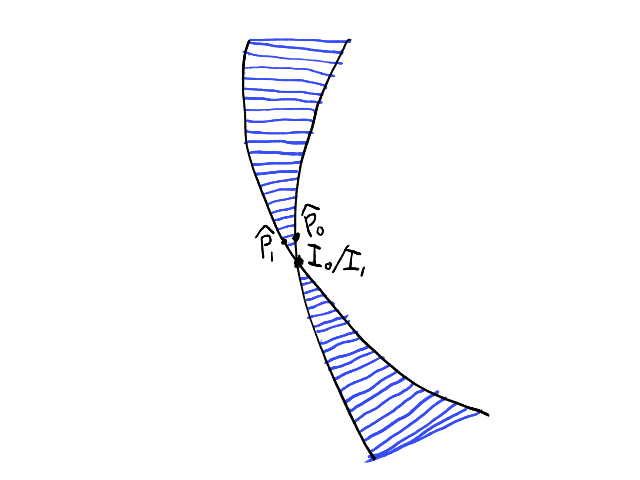
\includegraphics[scale=0.6]{5_inplace_ICP.png}
  \end{center}
  \caption{Iterative Closest Point (ICP), finding angle around $O_0$ and $O_1$}
	\label{fig:inplace_ICP}
\end{figure}

The result of the search gives us the components of the in-place transform we need for our constraint.  Given the pose of the two nodes at the end of the ICP search, we compute what the geometric transform would be between the two GPAC poses $\hat{P}_0$ and $\hat{P}_1$.  That gives us the transform component of the constraint.

Experimentally, we've determined that an effective covariance for the in-place constraint is:

\begin{equation}
C_{01} = 
\begin{bmatrix}
0.05 & 0 & 0 \\
0 & 0.05 & 0 \\
0 & 0 & \frac{\pi}{16}
\end{bmatrix}
\end{equation}


This indicates that the translational error is tight and equal in all directions.  However, the angular error is even tighter than in our motion constraint.  Experimentally, this is a very accurate relation between nodes in the pose graph.


%Compute B-Spline of segment posture of forward and backward nodes 
%local coordinates, local origin at $P_{19}$
%Find closest point on axis to local origin.
%Place each point on top of and tangent to each other
%Run ICP algorithm to find correct orientation
%Compute offset, add covariance, result is constraint


\subsection{Step Constraint}

The step constraint is an alternative to the motion constraint.  Instead of tracking reference poses and using the motion estimation subsystem to extract a geometric transform, we approximate a motion estimate by a fixed displacement along the direction of travel.  This estimate is the average displacement for each locomotion step of the snake.

There are a number of advantages to this approach.  Firstly, since we have already defined a forward and backward direction by derivation of the GPAC local coordinate frame, we have a clue of which direction the robot will travel.  Secondly, if we use this new approach, we are no longer concerned if error accumulates in our reference poses, since we no longer use them in estimating motion.

To create the step constraint, we use a similar approach to the in-place constraint.  We start with the two GPACs, $\beta_0^f(u)$ and $\beta_2^f(u)$ of the two nodes $v_0^f$ and $v_2^f$ and find their closest points $I_0$ and $I_2$ to the origins $O_0$ and $O_2$.  We solve for the $u_0$ and $u_2$ such that:
\begin{equation}
\beta_0^f(u_0) = I_0
\end{equation}
\begin{equation}
\beta_2^f(u_2) = I_2
\end{equation}
Just like the in-place constraint, we place the curves on top of each other such that $I_0 = I_2$.

In the next step, we differ from the in-place constraint.  Instead of keeping $I_0$ and $I_2$ intersected, we walk $\beta_2^f$ the length of the curve $\beta_0^f$ in the direction of the travel by the guessed distance while still intersecting at the point $I_0$.  The point of intersection on $\beta_2^f$ is moved along by an arc length of $0.3$, an estimated travel distance.

Similarly to the in-place constraint, the positions of the curves are constrained according to the following equation:
\begin{equation}
\beta_2^b(u_v) = I_0 +
\begin{bmatrix}
0 \\
0 \\
\theta_v
\end{bmatrix}
\end{equation}
Here, two parameters are varied by the ICP algorithm, $\theta_v$ for the relative orientation of the tangents at the curve intersections, and $u_v$ for the position on the $\beta_2^f$ curve that intersects point $I_0$ on curve $\beta_0^f$.  We perform a 2D iterative closest point such that a best fit overlap is found.  By varying the $u_v$ parameter, we allow for our $0.3$ displacement guess to be wrong and find a better fit if there are some curved features to match against.  Otherwise, it will tend to stay in the same neighborhood.  The system is shown in Figure \ref{fig:step_ICP}.

\begin{figure}
  \begin{center}
    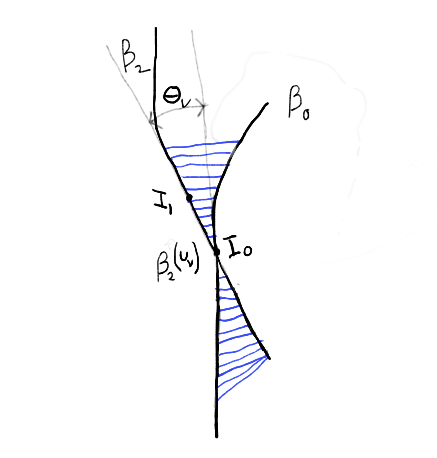
\includegraphics[scale=0.8]{5_step_ICP.png}
  \end{center}
  \caption{Iterative Closest Point (ICP), finding for $U_v$ and $\theta_v$ in step constraint}
	\label{fig:step_ICP}
\end{figure}

% From this displaced position, the angle of the relative orientation of the curves is rotated about $I_2$ until the best overlap is achieved by an iterative closest point (ICP) algorithm.

The geometric transform $T_{02}$ is extracted from their relative offset at the end of ICP search.  The covariance matrix is hand-made, of the form:

\begin{equation}
C_{02} = 
\begin{bmatrix}
0.1 & 0 & 0 \\
0 & 0.01 & 0 \\
0 & 0 & 0.02
\end{bmatrix}
\end{equation}

This indicates that we would expect to see more error along the axis of travel (forward-backward) with its covariance of $0.1$.  That is, the amount of displacement after each locomotion step is subject to more error than side-to-side.   In fact, the side-to-side error is an order of magnitude smaller because of our use of intersecting GPACs to guess motion, leaving little chance for sideways motion.   Similarly, the angular variance is also small since we ICP to keep the GPACs aligned. 

\section{Generalized ICP}

In two of the previous constraints, we used ICP to derive the appropriate geometric transform for the constraint.  We describe our approach to Iterative Closest Point.  We use a form of ICP called Generalized ICP \cite{}.

%@MISC{Segal_generalized-icp,
%    author = {Aleksandr V. Segal and Dirk Haehnel and Sebastian Thrun},
%    title = {Generalized-ICP},
%    year = {}
%}


\section{Results}

\subsection{Compare motion vs. step constraint}

Step more reliable, less variances in orientation which is most crucial

Good motion constraint requires slow movement of snake… not cheap.

Errors of motion are not easy to smooth out in pose graph

Use of step completely obviates need for self-posture motion estimation.  Only requires simple step motion model

\subsection{Alter estimate of step, show different results}

Characterized by error in translation, accuracy in orientation

